\begin{figure}
\centering
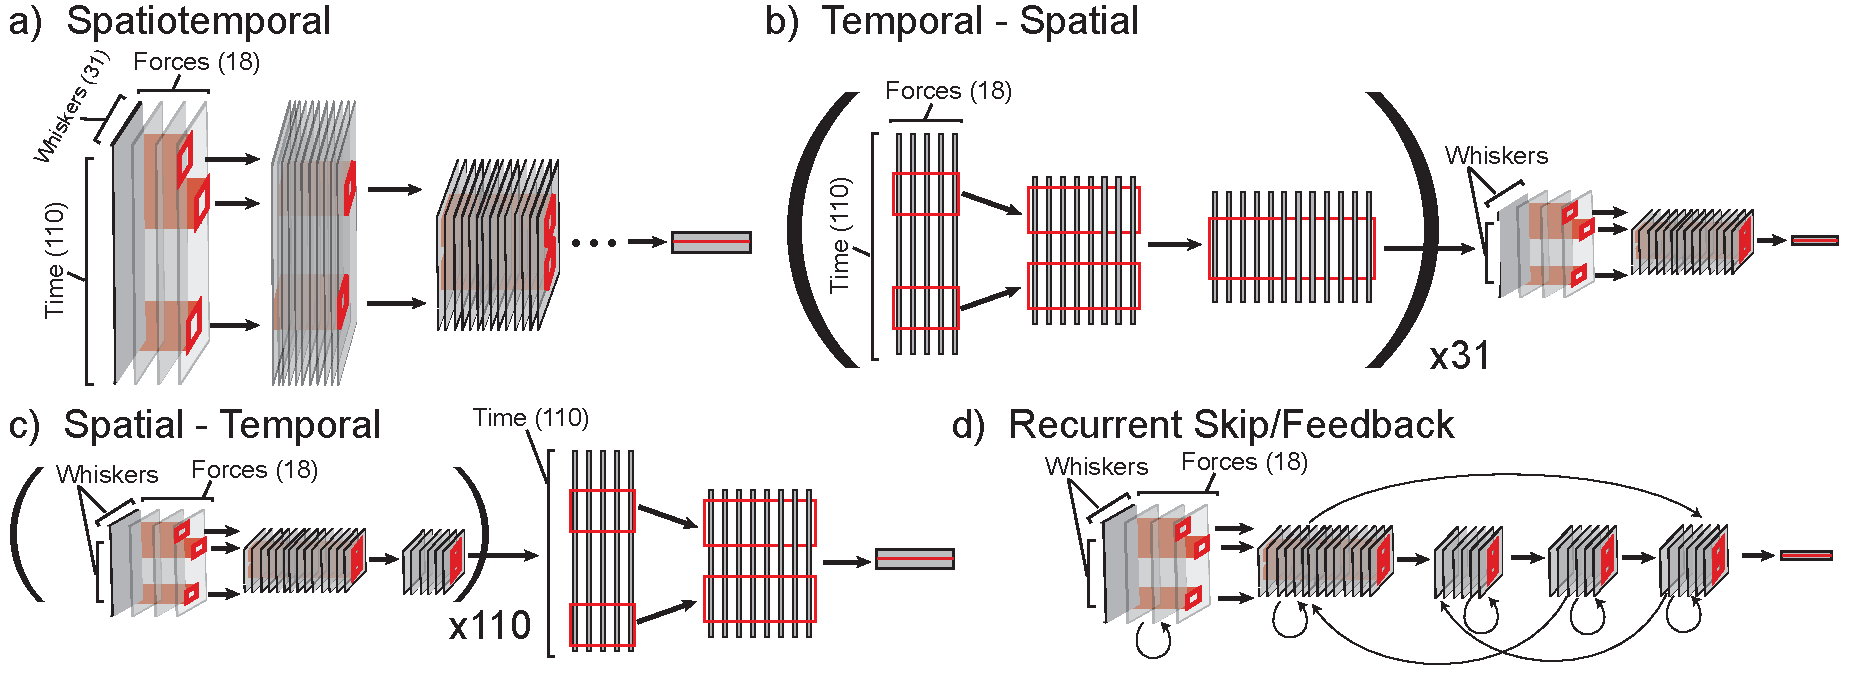
\includegraphics [width=1\linewidth]{figures/architectures.pdf}
\vspace{-2mm}
\caption{\textbf{Families of DNN Architectures tested:} \textbf{a.} ``Spatiotemporal'' models include spatiotemporal integration at all stages. Convolution is performed on both spatial and temporal data dimensions, followed by one or several fully connected layers. \textbf{b.} ``Temporal-Spatial'' networks in which temporal integration is performed separately before spatial integration.  Temporal integration consists of one-dimensional convolution over the temporal dimension, separately for each whisker. In spatial integration stages, outputs from each whisker are registered to their natural two-dimensional (2D) spatial grid and spatial convolution performed.  \textbf{c.} In ``Spatial-Temporal'' networks, spatial convolution is performed first, replicated with shared weights across time points; this is then followed by temporal convolution. \textbf{d.} Recurrent networks do not explicitly contain separate units to handle different discrete timepoints, relying instead on the states of the units to encode memory traces.  These networks can have local recurrence (e.g. simple addition or more complicated motifs like LSTMs or GRUs), as well as long-range skip and feedback connections.~\label{fig_archi}}
\end{figure}

We trained deep neural networks (DNNs) in a variety of different architectural families (Fig. \ref{fig_archi}).  
These architectures families can be thought of as representing qualitatively different classes of hypotheses about the computations performed by the stages of processing in the vibrissal-trigeminal system. 
The fundamental questions explored by these hypotheses are how and where temporal and spatial information are integrated.
Within each architectural family, the differences between specific parameter settings represent nuanced refinements of the larger hypothesis of that family.   
Parameter specifics include (e.g.) how many layers of each type are in the network, how many units are allocated to each layer, what kernel sizes are used at each layer, and so on.  
Biologically, these parameters may correspond to (e.g.) how many brain regions (areas) are in the cortex, how many neurons these regions have relative to each other, and neurons' local receptive field sizes~\cite{yamins2016using}.
 
\textbf{Simultaneous Spatiotemporal Integration.}
In this family of networks (Fig. \ref{fig_archi}a), networks consisted of convolution layers followed by one or more fully connected layers.  Convolution is performed simultaneously on both temporal dimension and spatial dimensions of the input (and their corresponding downstream dimensions). In other words, temporally proximal responses from spatially proximal whiskers are combined together simultaneously, so that neurons in each successive layers have larger receptive fields in both spatial and temporal dimensions at once.
We evaluated both 2D convolution, in which the spatial dimension is indexed linearly across the list of whiskers (first by vertical columns and then by lateral row on the $5\times7$ grid), as well as 3D convolution in which the two dimensions of the $5\times7$ spatial grid are explicitly represented.
Data from top, middle, and bottom sweep of the same object combined were to produce the final categorization, culminating in a standard softmax cross-entropy loss.  


\textbf{Separate Spatial and Temporal Integration.} In these families, networks begin by integrating temporal and spatial information separately (Fig. \ref{fig_archi}b-c).  
One subclass of these networks are ``Temporal-Spatial''  (Fig. \ref{fig_archi}b), which first integrate temporal information for each individual whisker separately and then combine the information from different whiskers in higher layers.
Temporal processing is implemented as 1-dimensional convolution over the temporal dimension. 
After several layers of temporal-only processing (the number of which is a parameter), the outputs at each whisker are then reshaped into vectors and combined into a $5\times7$ whisker grid.  Spatial convolutions are then applied for several layers. 
Finally, as with the spatiotemporal network described above, features from three sweeps are concatenated into a single fully connected layer which produces softmax category responses.

Conversely, ``Spatial-Temporal'' networks (Fig. \ref{fig_archi}c) first use 2D convolution to integrate across whiskers for some number of layers, with shared parameters between the copies of the network for each timepoint.  The temporal sequence of outputs is then combined, and several layers of 1D convolution are then applied in the temporal domain.  
Both Temporal-Spatial and Spatial-Temporal networks can be viewed as subclasses of 3D simultaneous spatiotemporal integration in which initial and final portions of the network have kernel size 1 in the relevant dimensions.  
These two network families can thus be thought of as two different strategies for allocating parameters between dimensions, i.e. different possible biological circuit structures.


\textbf{Recurrent Neural Networks with Skip and Feedback Connections.} This family of networks (Fig. \ref{fig_archi}d) does not allocate units or parameters explicitly for the temporal dimension, and instead requires temporal processing to occur via the temporal update evolution of the system.  These networks are built around a core feedforward 2D spatial convolution structure, with the addition of (i) local recurrent connections, (ii) long-range feedforward skips between non-neighboring layers, and (iii) long-range feedback connections.  
The most basic update rule for the dynamic trajectory of such a network through (discrete) time is: 
$$H^i_{t+1} = F_i \left ( \oplus_{j \neq i} R^j_t \right )  + \tau_i H^i_t \quad ;\quad R^i_t = A_i[H^i_t]$$
where $R^i_t$ and $H^i_t$ are the output and hidden state of layer $i$ at time $t$ respectively,  $\tau_i$  are decay constants, $\oplus$ represents concatenation across the channel dimension with appropriate resizing to align dimensions, $F_i$ is the standard neural network update function (e.g. 2-D convolution), and $A_i$ is activation function at layer $i$.  
The learned parameters of this type of network include the values of the parameters of $F_i$, which comprises both the feedforward and feedback weights from connections coming in to layer $i$, as well as the decay constants $\tau_i$. 
More sophisticated dynamics can be incorporated by replacing the simple additive rule above with a local recurrent structure such as Long Short-Term Memory (LSTM)~\cite{Hochreiter1997} or Gated Recurrent Networks (GRUs)~\cite{cho2014properties}.


